\documentclass{beamer}
\usepackage{etex}

%\useoutertheme[glossy]{wuerzburg}
\useinnertheme[shadow,outline]{chamfered}
%\usecolortheme{shark}
\usecolortheme{beaver}
\beamertemplatenavigationsymbolsempty

\usefonttheme{professionalfonts}
\let\digamma\relax
\usepackage[scale=0.85,stdmathitalics=true,romanfamily=casual]{lucimatx}
\usefonttheme[stillsansseriftext]{serif}



\usepackage{fancyvrb}

%% Fancy syntax coloring via pygments
\usepackage{minted}
\definecolor{bg}{rgb}{0.95,0.95,0.95}
\usemintedstyle{borland}


\newenvironment{Rcode}
{\VerbatimEnvironment
 \begin{minted}[fontsize=\scriptsize,baselinestretch=1]{r}}%
{\end{minted}}

\newenvironment{Pcode}
{\VerbatimEnvironment
 \begin{minted}[fontsize=\scriptsize,baselinestretch=1]{python}}%
{\end{minted}}

\newenvironment{Code}[1]
{\VerbatimEnvironment
 \begin{minted}[fontsize=\scriptsize,baselinestretch=1]{#1}}%
{\end{minted}}


\usepackage{textfit} % commands \scaletoheight{height}{text} and \scaletowidth{width}{text}

\usepackage{tikz}

\usepackage{tcolorbox}

\newtheorem{Alert}{Alert}
\newtheorem{Highlight}{Highlight}

\newcommand{\Species}[1]{{\rmfamily \itshape #1}}
\newcommand{\Real}{\ensuremath{\mathbb{R}}}
\newcommand{\RealN}{\ensuremath{\mathbb{R}^n}}
\newcommand{\RealP}{\ensuremath{\mathbb{R}^p}}
\newcommand{\Mtx}[1]{\ensuremath{\mathbf{#1}}}
\newcommand{\Inv}[1]{\ensuremath{#1^{-1}}}
\newcommand{\InvMtx}[1]{\ensuremath{\mathbf{#1}^{-1}}}
\newcommand{\Red}[1]{\textcolor{red}{#1}}
\newcommand{\PsInv}[1]{\ensuremath{\mathbf{#1}^{+}}}

\usepackage{booktabs}



% --- Macro \xvec
% From a tex.stackexchange.com answer by Todd Lehman
% http://tex.stackexchange.com/questions/44017/dot-notation-for-derivative-of-a-vector
\makeatletter
\newlength\xvec@height%
\newlength\xvec@depth%
\newlength\xvec@width%
\newcommand{\xvec}[2][]{%
  \ifmmode%
    \settoheight{\xvec@height}{$#2$}%
    \settodepth{\xvec@depth}{$#2$}%
    \settowidth{\xvec@width}{$#2$}%
  \else%
    \settoheight{\xvec@height}{#2}%
    \settodepth{\xvec@depth}{#2}%
    \settowidth{\xvec@width}{#2}%
  \fi%
  \def\xvec@arg{#1}%
  \def\xvec@dd{:}%
  \def\xvec@d{.}%
  \raisebox{.2ex}{\raisebox{\xvec@height}{\rlap{%
    \kern.05em%  (Because left edge of drawing is at .05em)
    \begin{tikzpicture}[scale=1]
    \pgfsetroundcap
    \draw (.05em,0)--(\xvec@width-.05em,0);
    \draw (\xvec@width-.05em,0)--(\xvec@width-.15em, .075em);
    \draw (\xvec@width-.05em,0)--(\xvec@width-.15em,-.075em);
    \ifx\xvec@arg\xvec@d%
      \fill(\xvec@width*.45,.5ex) circle (.5pt);%
    \else\ifx\xvec@arg\xvec@dd%
      \fill(\xvec@width*.30,.5ex) circle (.5pt);%
      \fill(\xvec@width*.65,.5ex) circle (.5pt);%
    \fi\fi%
    \end{tikzpicture}%
  }}}%
  #2%
}
\makeatother

% --- Override \vec with an invocation of \xvec.
\let\stdvec\vec
\renewcommand{\vec}[1]{\xvec[]{#1}}
% --- Define \dvec and \ddvec for dotted and double-dotted vectors.
\newcommand{\dvec}[1]{\xvec[.]{#1}}
\newcommand{\ddvec}[1]{\xvec[:]{#1}}


\usepackage{pifont}
\newcommand{\weblink}{\ding{43}}  % hand with pointing finger

\definecolor{links}{HTML}{2A1B81}
\hypersetup{colorlinks,linkcolor=,urlcolor=magenta}

\usepackage{tikz}

\usepackage{amsfonts}
\usepackage{tikz}
\usepackage{caption}
\usepackage{subcaption}

\usepackage[inline]{asymptote}
\usepackage{attachfile2}
\usepackage{asyfig}




%===========================================================
% Title Info
\title{Scientific Computing for Biologists}
\subtitle{Linear Algebra Review II \& Multiple Regression} % (optional)

\author{Instructor: Paul M. Magwene}


\date{17 September 2013}

\begin{document}
%===========================================================
\begin{frame}
\titlepage
\end{frame}

%===========================================================
\begin{frame}
  \frametitle{Overview of Lecture}

\begin{itemize}
		\item More Linear Algebra
		\begin{itemize}
			\item Linear combinations and Spanning Spaces
			\item Subspaces
			\item Basis vectors
			\item Dimension
			\item Rank
		\end{itemize}
		\item More on Regression
		\begin{itemize}
		  \item Multiple regression
		  \item Curvilinear regression
		  \item Major axis regression
		\end{itemize}
\end{itemize}

\end{frame}
%===========================================================

%===========================================================
\begin{frame}
  \frametitle{Hands-on Session}
\begin{itemize}
    \item Multiple regression
\end{itemize}


\end{frame}
%===========================================================



%===========================================================
\begin{frame}[fragile]
  \frametitle{A bit of review}

\begin{center}
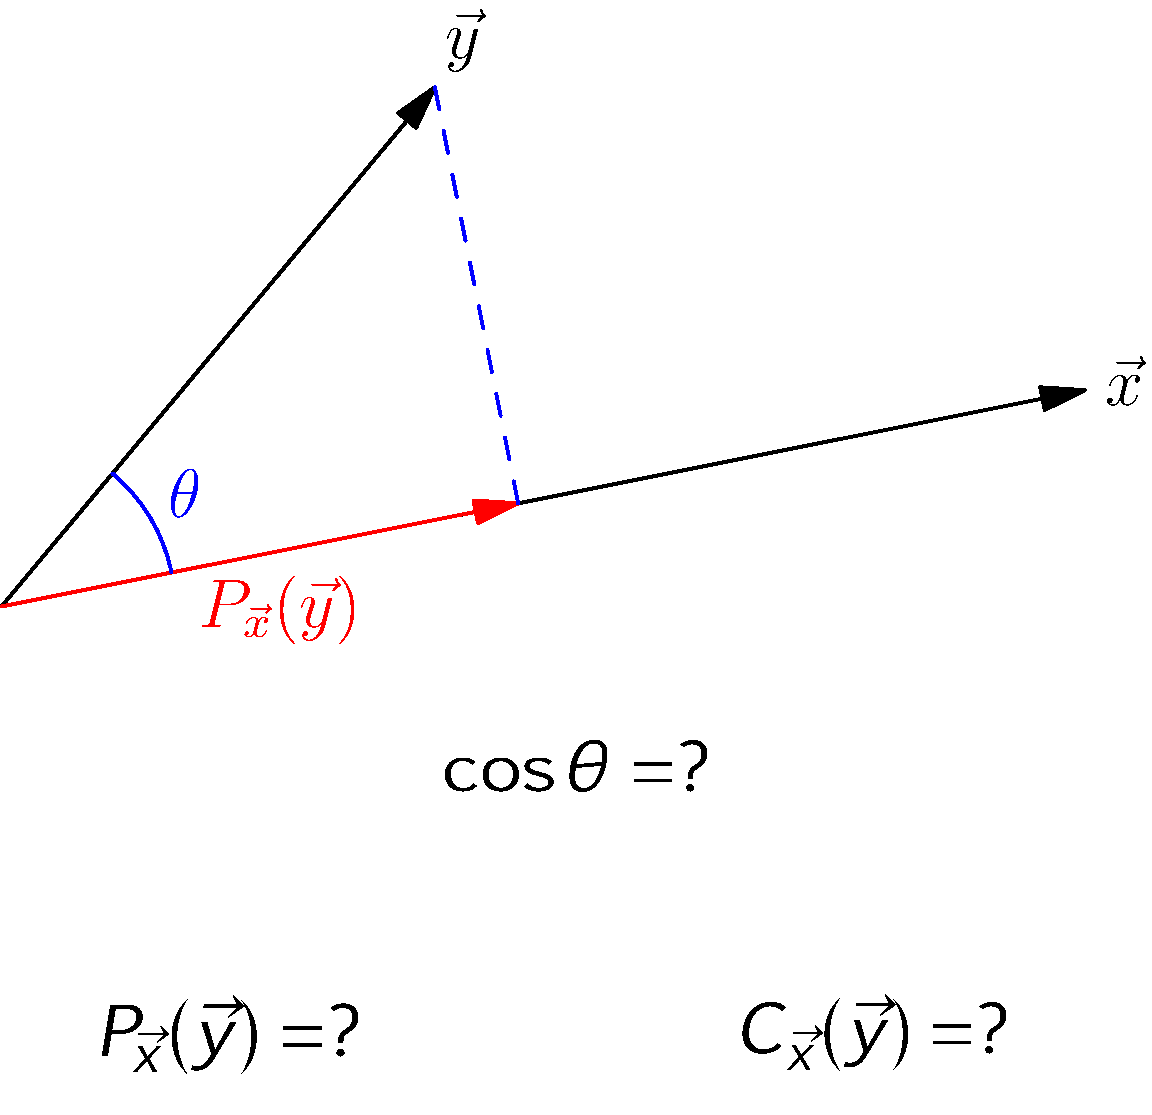
\includegraphics[width=0.65\textwidth]{geomreview.pdf}
\end{center}

\end{frame}
%===========================================================



%===========================================================
\begin{frame}
  \frametitle{Space Spanned by a List of Vectors}


\begin{block}{Definition}

Let $X$ be a finite list of $n$-vectors. The \textbf{space spanned} by $X$ is the set of all vectors that can be written as linear combinations of the vectors in $X$.
\medskip

A space spanned includes the zero vector and is closed under addition and multiplication by a scalar.

\end{block}
\bigskip

Remember that a \emph{linear combination} of vectors is an equation of the form $z = b_1 \Mtx{x}_1 + b_2 \Mtx{x}_2 + \cdots + b_p \Mtx{x}_p$

\end{frame}

%===========================================================


%===========================================================
\begin{frame}
  \frametitle{Subspaces}

$\RealN$  denotes the seat of real $n$-vectors - the set of all $n \times 1$ matrices with entries from the set $\Real$ of real numbers.
\medskip

\begin{block}{Definition}

A \textbf{subspace} of $\Real^n$ is a subset S of $\Real^n$ with the following properties:
\begin{enumerate}
	\item $\Mtx{0} \in S$
	\item If $\Mtx{u} \in S$ then $k\Mtx{u} \in S$ for all real numbers $k$
	\item If $\Mtx{u} \in S$ and  $\Mtx{v} \in S$ then $\Mtx{u} + \Mtx{v} \in S$
\end{enumerate}

\end{block}

Examples of subspaces of $\Real^n$:
\begin{itemize}
	\item any space spanned by a list of vectors in $\Real^n$
	\item the set of all solutions to an equation $A\Mtx{x} = \Mtx{0}$ where $A$ is a $p \times n$ matrix, for any number p.
\end{itemize}

\end{frame}
%===========================================================

%===========================================================
\begin{frame}
  \frametitle{Basis}

Let $S$ be a subspace of \RealN.  Then there is a finite list, $X$, of vectors from $S$ such that $S$ is the space spanned by $X$.
\medskip

Let $S$ be a subspace of $\RealN$ spanned by the list $(u_1, u_2, \ldots, u_n)$. Then  there is a linearly independent sublist of $(u_1, u_2, \ldots, u_n)$ that also spans $S$.
\medskip

\begin{block}{Definition}
A list $X$ is a \textbf{basis} for $S$ if:
\begin{itemize}
\item $X$ is linearly independent
\item $S$ is the subspace spanned by $X$
\end{itemize}
\end{block}

\end{frame}
%===========================================================

%===========================================================
\begin{frame}
  \frametitle{Dimension}
Let $S$ be a subspace of \RealN.
\bigskip

\begin{block}{Definition}
The \textbf{dimension} of $S$ is the number of elements in a basis for $S$.
\end{block}

\end{frame}
%===========================================================


%===========================================================
\begin{frame}
  \frametitle{Rank of a Matrix}
Let $A$ by an $n \times p$ matrix.
\bigskip

\begin{block}{Definition}
The \textbf{rank} of $A$ is equal to the dimension of the row space of $A$ which is equal to the dimension of the column space of $A$.
\end{block}
\bigskip
Where the row space of $A$ is the space spanned by the list of rows of $A$ and the column space of $A$ is defined similarly.

\end{frame}
%===========================================================

% %===========================================================
% \begin{frame}
%   \frametitle{Equivalence Theorem}
% Let $A$ by an $p \times p$ matrix. The following are equivalent
% \medskip

% \begin{itemize}
% 	\item $A$ is singular
% 	\item the rank of $A$ is less than $p$
% 	\item the columns of $A$ form a LD list in \RealN.
% 	\item the rows of $A$ form a LD list in \RealN
% 	\item the equation $A\Mtx{x} = \Mtx{0}$ has non-trivial solutions
% 	\item the determinant of $A$ is zero
% \end{itemize}

% \end{frame}

%===========================================================

\begin{frame}
  \frametitle{}

\begin{center}
\begin{Huge}
Regression Models
\end{Huge}
\end{center}
\end{frame}

%===========================================================
\begin{frame}[fragile]
  \frametitle{Variable space view of multiple regression}

\begin{center}
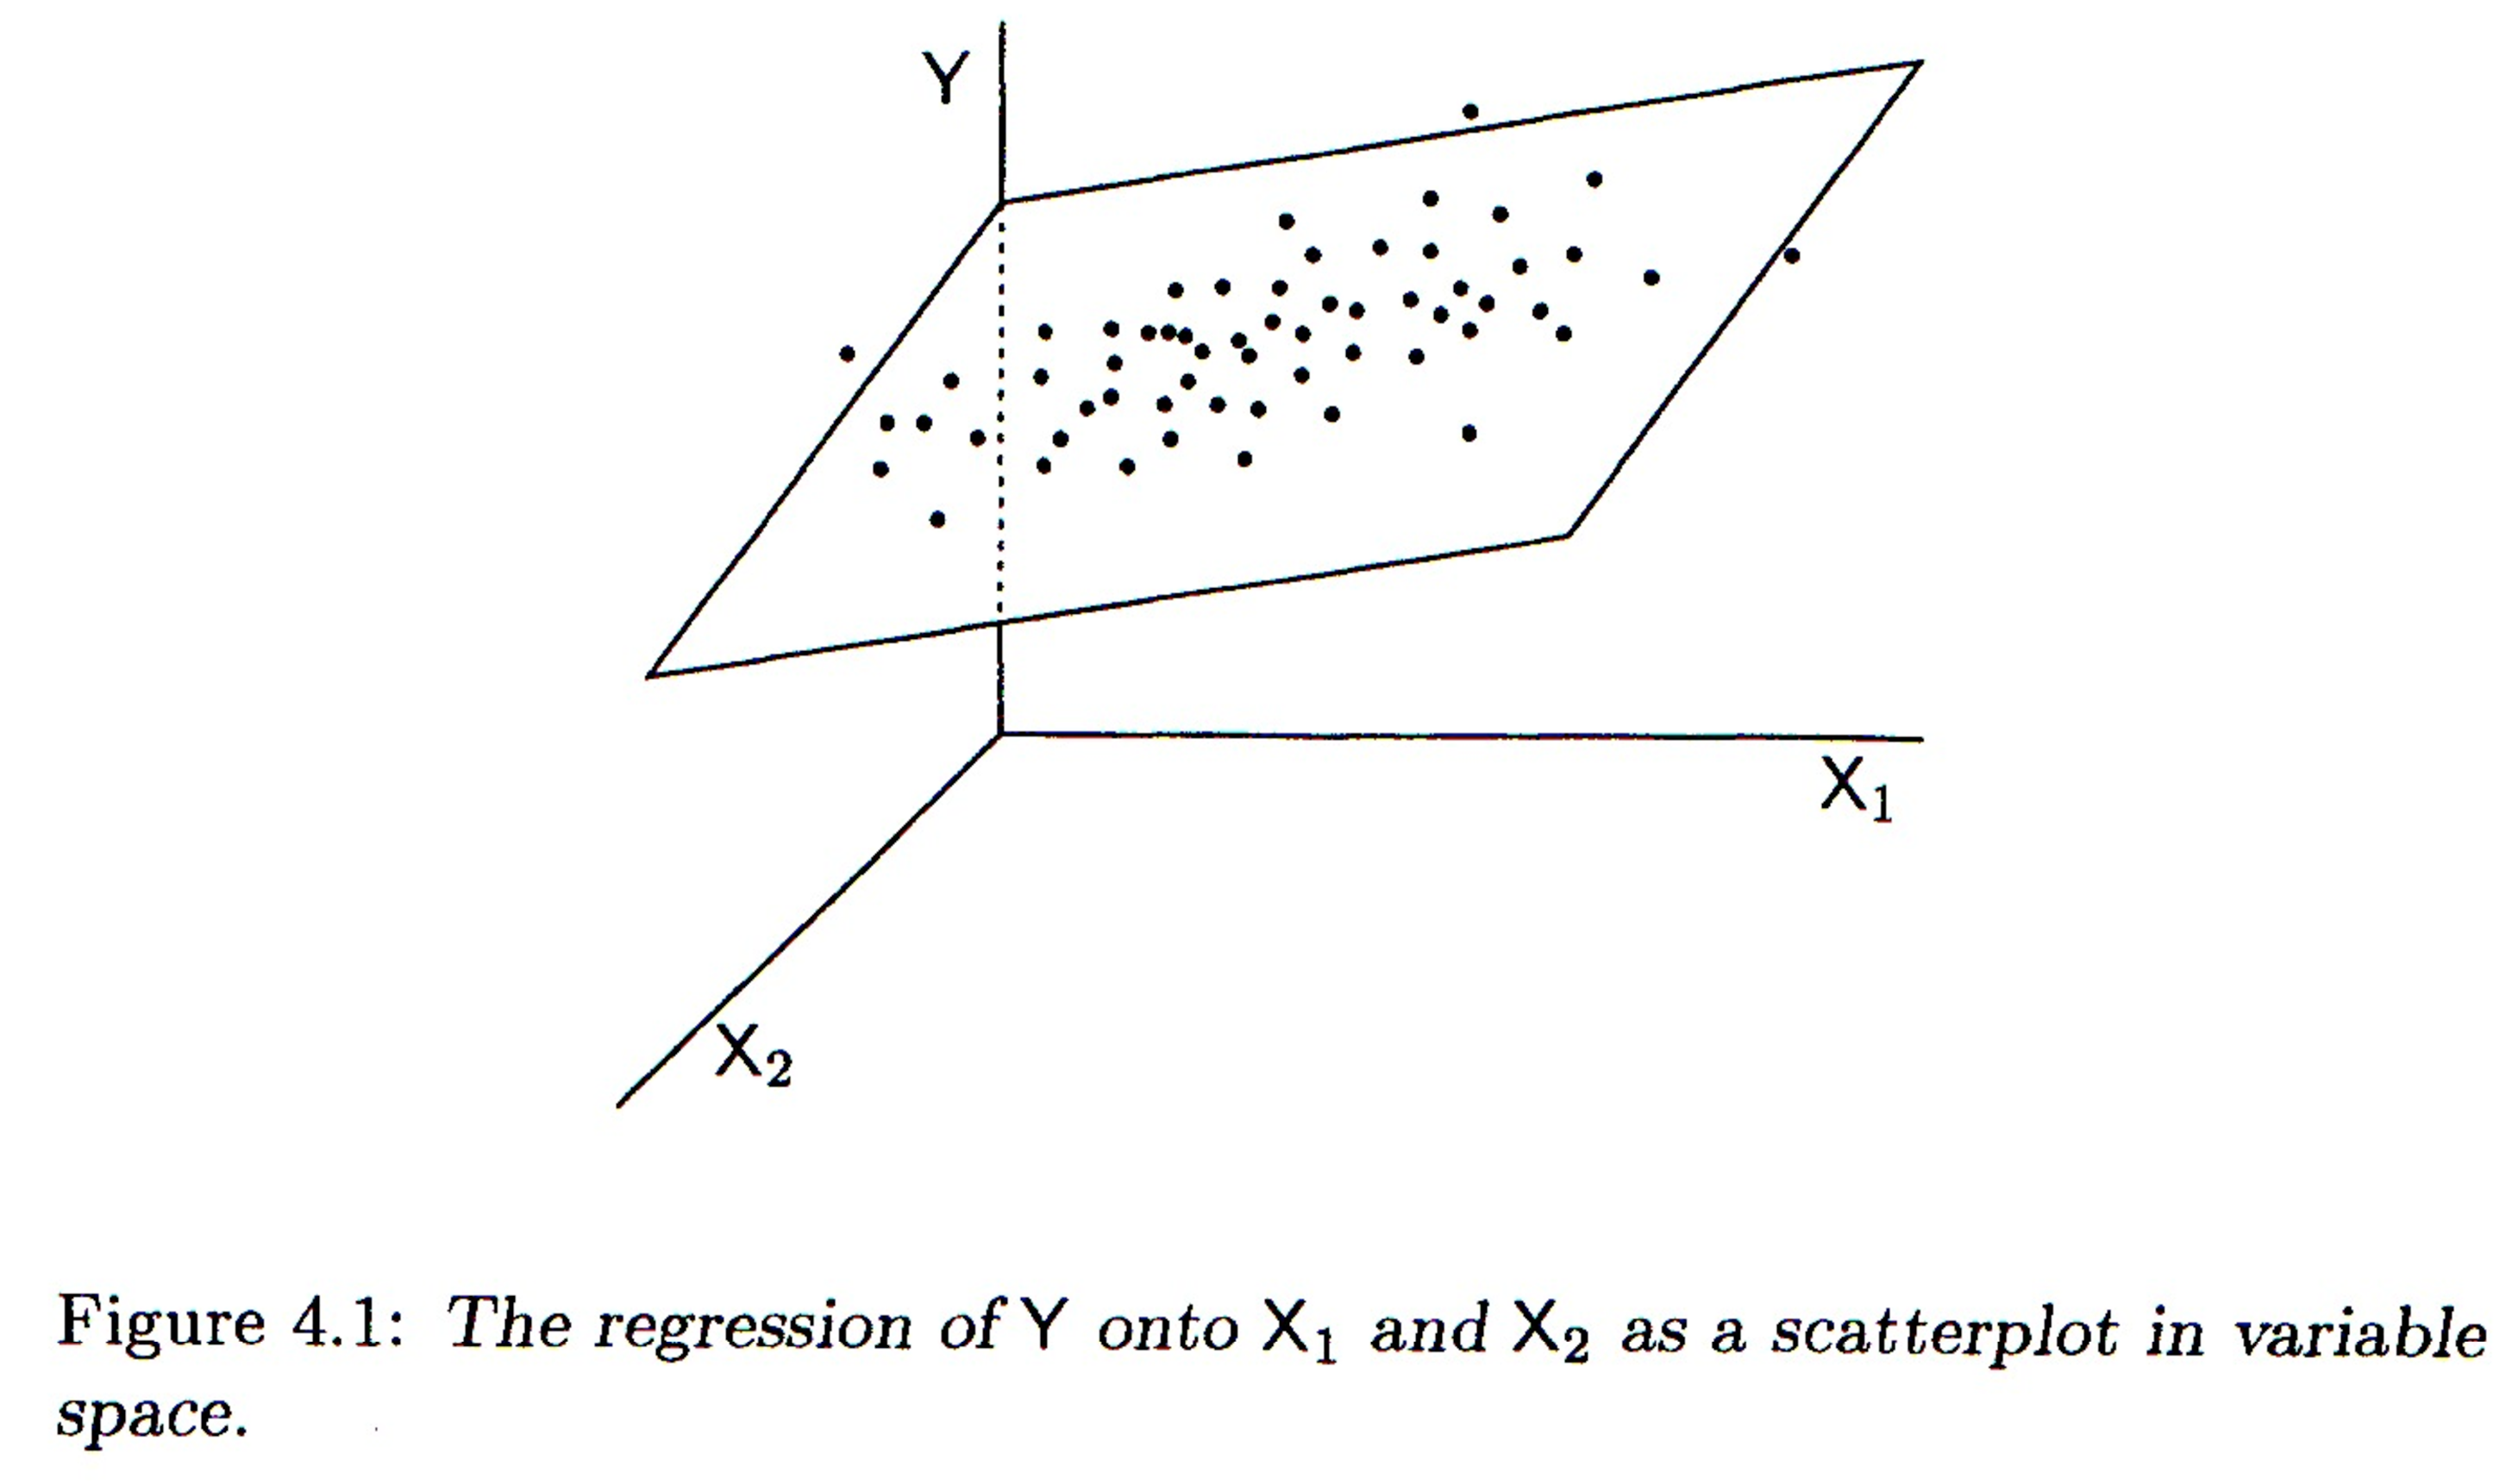
\includegraphics[height=2.5in]{regression-variable-space}
\end{center}


\end{frame}
%===========================================================


%===========================================================
\begin{frame}
  \frametitle{Subject Space Geometry of Multiple Regression}

\begin{center}
\asyinclude[height=2.5in,inline=true]{multiregr.asy}
%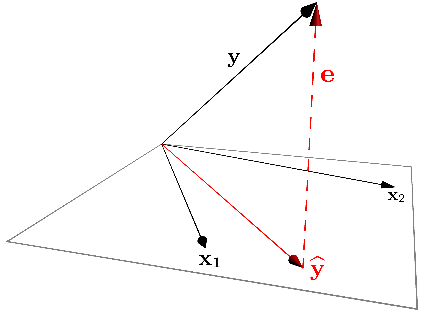
\includegraphics[height=2.5in]{multiregr.pdf}

\end{center}
\end{frame}

%===========================================================
\begin{frame}
  \frametitle{Multiple Regression}

Let $Y$ be a vector of values for the outcome variable. Let $\Mtx{X}_i$ be explanatory variables and let $\Mtx{x}_i$ be the mean-centered explanatory variables.
\medskip

$$
\Mtx{Y} = \hat{\Mtx{Y}} + \Mtx{e}
$$
where --
\bigskip

Uncentered version:
$$
\hat{Y} = a\Mtx{1} + b_1\Mtx{X}_1 + b_2\Mtx{X}_2 + \cdots + b_p\Mtx{X}_p
$$

Centered version:
$$
\hat{y} = b_1\Mtx{x}_1 + b_2\Mtx{x}_2 + \cdots + b_p\Mtx{x}_p
$$


\end{frame}
%===========================================================
\begin{frame}
  \frametitle{Statistical Model for Multiple Regression}

In matrix form:

$$
\Mtx{y} = \Mtx{X}\Mtx{b} + \Mtx{e}
$$

$$
\Mtx{y} = \left[ \begin{array}{c}
y_1 \\ y_2 \\ \vdots \\y_n \\
\end{array}
\right]
\;
;
\;
\Mtx{X} = \left[ \begin{array}{ccccc}
1 & x_{11} & x_{12} & \cdots & x_{1p} \\
1 & x_{21} & x_{22} & \cdots & x_{2p} \\
\vdots & \vdots & \vdots & \vdots & \vdots \\
1 & x_{n1} & x_{n2} & \cdots & x_{np} \\
\end{array}
\right]
\;
;
$$

$$
\Mtx{b} = \left[ \begin{array}{c}
a \\ b_1 \\ b_2 \\ \vdots \\ b_p \\
\end{array}
\right]
\;
;
\;
\Mtx{e} = \left[ \begin{array}{c}
e_1 \\ e_2 \\ \vdots \\e_n \\
\end{array}
\right]
$$

\end{frame}
%===========================================================
\begin{frame}
  \frametitle{Estimating the Coefficients for Multiple Regression}


$$
\Mtx{y} = \Mtx{X}\Mtx{b} + \Mtx{e}
$$
\bigskip

Estimate \Mtx{b} as:
$$
\Mtx{b} = (\Mtx{X}^T \Mtx{X})^{-1}\Mtx{X}^T\Mtx{y}
$$

\end{frame}
%===========================================================
\begin{frame}
  \frametitle{Multiple Regression Loadings}


The regression \textbf{loadings} should be examined as well as the regression coefficients.

\begin{center}
\asyinclude[viewportwidth=0.3\textwidth,height=1.5in,keepAspect=true,inline=true]{multiregr-loadings.asy}
%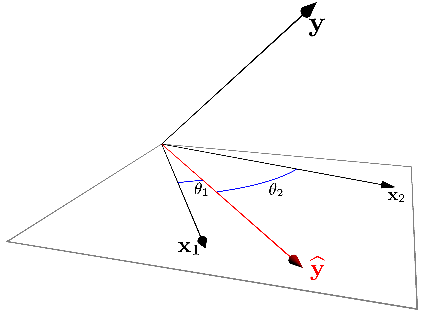
\includegraphics[height=1.5in]{multiregr-loadings.pdf}
\end{center}

Loadings are given by:
		\[
		\cos \theta_{\vec{x_j},\vec{\widehat{y}}} = \frac{\vec{x_j} \cdot \vec{\widehat{y}}}{|\vec{x_j}||\vec{\widehat{y}}|}
		\]


\end{frame}




%===========================================================
\begin{frame}
  \frametitle{Multiple regression: Cautions and Tips}


\begin{itemize}
    \item Comparing the size of regression coefficients only makes sense if all the predictor variables have the same scale
	\item The predictor variables  (columns of $\Mtx{X}$) must be linearly independent; when they're not the variables are \textbf{multicollinear}
	\item Predictor variables that are \textbf{nearly multicollinear} are, perhaps, even more difficult to deal with
\end{itemize}

\end{frame}

%===========================================================

\begin{frame}
  \frametitle{Why is near multicollinearity of the predictors a problem?}

\begin{figure}
\begin{center}
\subcaptionbox{Non-collinear predictors}{\asyinclude[height=1.35in,keepAspect=true]{regr-noncolinear.asy}}
%{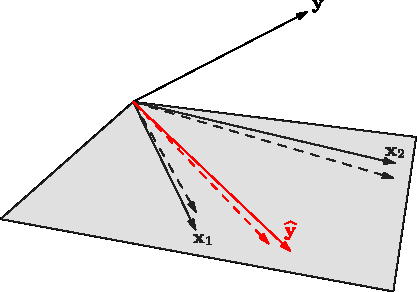
\includegraphics[height=1.25in]{regr-noncolinear.pdf}}
\subcaptionbox{Nearly collinear predictors}{\asyinclude[height=1.35in,keepAspect=true]{regr-colinear.asy}}
%{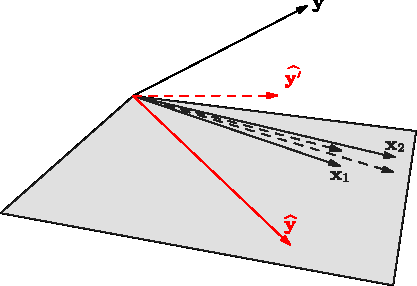
\includegraphics[height=1.25in]{regr-colinear.pdf}}
\end{center}
\caption{When predictors are nearly collinear, small differences in the vectors can result in large differences in the estimated regression.}
\end{figure}


\end{frame}

%===========================================================

\begin{frame}
  \frametitle{What can I do if my predictors are (nearly) collinear?}

\begin{itemize}
	\item Drop some of the linearly dependent sets of predictors.
	\item Replace the linearly dependent predictors with a combined variable.
	\item Define orthogonal predictors, via linear combinations of the original variables (PC regression approach)
	\item `Tweak' the predictor variables so that they're no longer multicollinear (Ridge regression).
\end{itemize}


\end{frame}




%===========================================================
\begin{frame}
  \frametitle{Curvilinear Regression}

Curvilinear regression using \textbf{polynomial models} is simply multiple regression with the $x_i$ replace by powers of $x$.
\bigskip

$$
\hat{y} = b_1\Mtx{x} + b_2\Mtx{x}^2 + \cdots + b_p\Mtx{x}^n
$$

\medskip

Note:
\begin{itemize}
	\item this is still a \emph{linear} regression (linear in the coefficients)
	\item best applied when a specific hypothesis justifies there use
	\item generally not higher than quadratic or cubic
\end{itemize}

\end{frame}
%===========================================================
\begin{frame}[fragile]
  \frametitle{Example of Curvilinear Regression}

\begin{center}
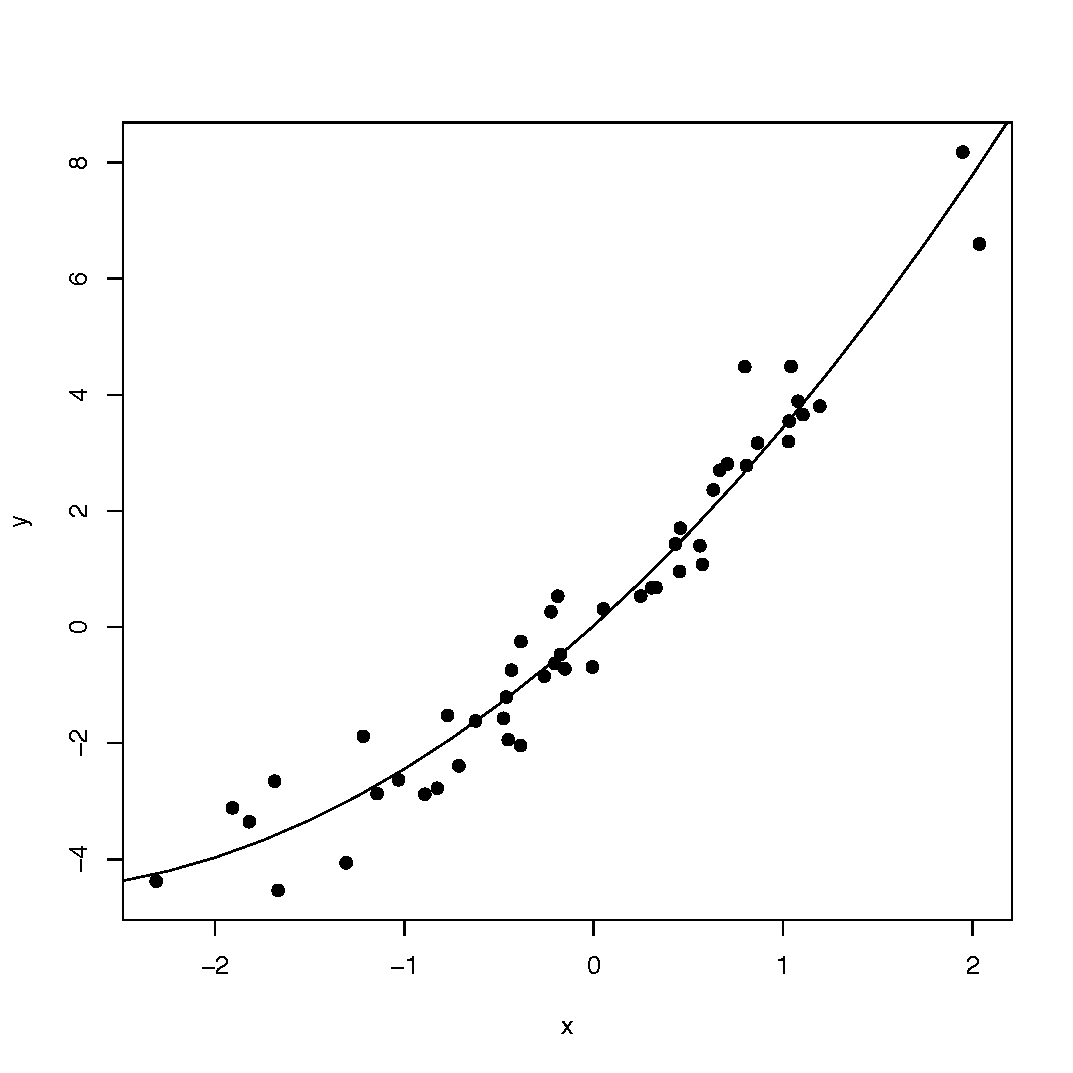
\includegraphics[height=1.75in]{curvilinear}\\
 $\Mtx{y} = 3\Mtx{x} + 0.5\Mtx{x}^2 + \Mtx{e}$
\end{center}

\begin{Rcode}
lm(formula = y ~ x + I(x^2))
Coefficients:
            Estimate Std. Error t value Pr(>|t|)
(Intercept)  0.02229    0.11651   0.191    0.849
x            2.94001    0.09693  30.331  < 2e-16 ***
I(x^2)       0.47146    0.07685   6.135 1.68e-07 ***
\end{Rcode}


\end{frame}


%===========================================================

\begin{frame}
  \frametitle{Least Squares Regression vs. Major Axis Regression}
\begin{center}
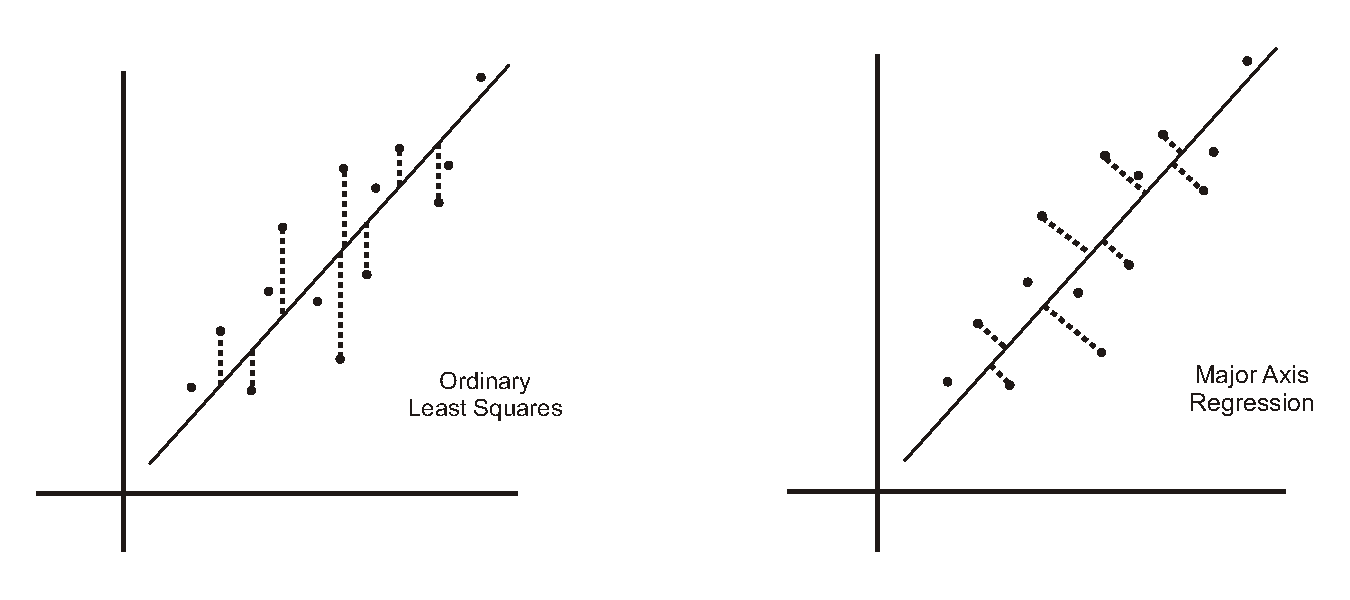
\includegraphics[width=4in]{ols_vs_majoraxis}
\end{center}
\end{frame}


%===========================================================


\begin{frame}
  \frametitle{Vector Geometry of Major Axis Regression}

\begin{figure}
\begin{center}
\subcaptionbox{OLS}{{\asyinclude[height=1.05in,keepAspect=true]{geom-OLS.asy}}}
%{\includegraphics[height=1.05in]{geom-OLS.pdf}}
\subcaptionbox{Major Axis Regression}{{\asyinclude[height=1.05in,keepAspect=true]{geom-majaxis.asy}}}
%{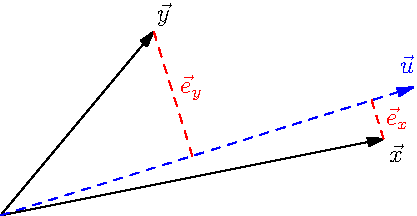
\includegraphics[height=1.05in]{geom-majaxis.pdf}}
\end{center}
\caption{Vector geometry of ordinary least-squares and major axis regression.}
\end{figure}


\end{frame}

%===========================================================



\end{document}


%===========================================================
\begin{frame}
  \frametitle{XXX}

\end{frame}
%===========================================================
